% !TEX root = Hauptdatei.tex
\section{Einleitung}\label{einleitung}

%Stichworte
% - Ausganssituation
% 
% Aufgabenstellung + Ziel -> Konzeption und Umsetzung eines HMI Konzepts für Instrument Cluster auf Basis von Linux
% Beschreibung technisches Umfeld/Voraussetzungen

%Anmerkungen von Andi: Emotionaler, Entwicklung HMI komplexität von technik, Warum braucht man HMI, mehr text unter den bildern, nicht schlimm wenn man sich wiederholt


% Titel der Arbeit aufnehmen und anfangen zu erklären
% Worum gehts?
% Was ist ein Kombiinstrument
% Welche Funktionen erfüllt es
% Wo geht die Entwicklung hin



%Was ist ein \ac{HMI}? In das Deutsche übersetzt Mensch-Maschine-Schnittstelle.
Was ist ein \acf{HMI}? 

Human-Machine-Interface ist eine Wortzusammensetzung aus drei Wörtern, Human (Mensch), Machine (Maschine) und Interface (Schnittstelle).\\

%Definition Mensch nach Duden
Der Duden definiert Mensch als ein, \glqq mit der Fähigkeit zu logischem Denken und zur Sprache, zur sittlichen Entscheidung und Erkenntnis von Gut und Böse ausgestattetes höchstentwickeltes Lebewesen\grqq{} \cite{duden_mensch}.\\

%Definition Maschine Duden
Eine Maschine wird als, \glqq mechanische, aus beweglichen Teilen bestehende Vorrichtung, die Kraft oder Energie überträgt und mit deren Hilfe bestimmte Arbeiten unter Einsparung menschlicher Arbeitskraft ausgeführt werden können\grqq{} definiert \cite{duden_maschine}.\\

%Definition Schnittstelle Duden
Eine Schnittstelle ist laut Duden eine \glqq Verbindungsstelle zwischen Funktionseinheiten eines Datenverarbeitungs- oder -übertragungssystems, an der der Austausch von Daten oder Steuersignalen erfolgt \grqq{} \cite{duden_schnittstelle}.\\

Maschinen verrichten Arbeiten die für Menschen nur schwer oder gar nicht durchführbar sind. In der Regel haben Maschinen nicht die Fähigkeit logisch zu denken. Daher wird zwischen Menschen und Maschinen eine Schnittstelle benötigt. Diese Schnittstelle ist für den Datenaustausch zuständig. Bei \acp{HMI} wird aber nicht zwingend nur mit Maschinen interagiert sondern auch mit Geräten. Geräte führen nicht zwangsläufig Arbeiten durch bei denen Kraft benötigt wird, jedoch erleichtern sie bestimmte Aufgaben für den Menschen. Als Beispiel für ein Gerät zählt beispielsweise ein Computer oder Smartphone. Diese Geräte erleichtern den Zugang zum Internet oder die Kommunikation mit anderen Menschen an anderen Orten.\\

Aus diesen verschiedenen Bedeutungen ergibt sich für \aclp{HMI} folgende Definition:\\

%Definition HMI
\textit{
Ein Human-Machine-Interface bietet eine Schnittstelle zwischen Mensch und Maschine. Es bündelt die Informationen der Maschine und bereitet diese für den Menschen auf. Mit Hilfe der Informationen kann der Mensch die Maschine überwachen und bedienen.}\\
%Definition HMI

Ein sehr einfaches Beispiel für ein \ac{HMI} ist ein Lichtschalter, wie in Abbildung \ref{fig:gra_hmi} zu sehen ist. Der Lichtschalter gehört weder zum Menschen noch zur Lampe. Er ist lediglich die Schnittstelle dazwischen. Der Mensch kann dadurch mit der Lampe interagieren und sie ein- und ausschalten. Gleichzeitig bekommt der Mensch, über die Schalterstellung, die Information in welchem Zustand sich die Lampe befindet. \cite{wiki_schnittstelle}\\

\begin{figure}[htb]
	\centering
	
\includegraphics[width=13.5cm]{img/1_einleitung/HMI_Farbe}
	\caption{Grafische Darstellung eines \ac{HMI}}
	\label{fig:gra_hmi}
\end{figure}

Es gibt deutlich komplexere \acp{HMI} als einen Lichtschalter, da es deutlich komplexere Maschinen gibt und die Komplexität immer weiter steigt. Einige Maschinen lassen sich ohne aufwendige Interfaces nicht mehr bedienen. Das setzt allerdings auch ein immer größeres Hintergrundwissen derer Menschen voraus, welche die Maschinen bedienen.\\

\subsection{Geschichte von HMIs im automotive Bereich}
Die Geschichte und Entwicklung von \acp{HMI} wird in diesem Kapitel anhand von verschiedenen Beispielen erläutert. Wie im vorherigen Teil beschrieben, ist etwa ein Lichtschalter eine sehr einfache Schnittstelle. In Fahrzeugen wurden schon immer Schnittstellen benötigt, allerdings haben sich die Anzahl und die Umsetzung über die Jahre stark verändert.\\

Während den Anfängen des Automobils gab es unter anderem Schnittstellen, die heute nicht mehr benötigt werden. Dazu zählt unter anderem die Zündzeitpunktverstellung. Jedoch gab es auch damals Schnittstellen, die heute noch in gleicher oder ähnlicher Form existieren.\\

Schon beim allerersten Automobil war es nötig die Richtung der Bewegung zu bestimmen. Daher war auch im ersten Automobil von Carl Benz ein Lenkhebel verbaut. Ein Lenhebel zeigt an in welche Richtung gefahren wird. Durch drehen am Lenhebel lässt sich die Richtung ändern in die sich das Fahrzeug bewegt. Der Lenkhebel wurde später durch das Lenkrad ersetzt. Außerdem war es möglich die Geschwindigkeit zu verändern. Beim Benz Patent-Motorwagen Nummer 1 wurde die Abgabeleistung und damit die Geschwindigkeit noch mit einem Hülsenschieber geregelt. Heute wird das, über das Gaspedal und einen Bowdenzug, oder elektronisch geregelt.\\%cite wikipedia benz patent motor wagen nummer 1

Mit der Zeit veränderten sich die Schnittstellen und neue Schnittstellen kamen hinzu. Nicht mehr benötigte Schnittstellen wurden entfernt und die wichtigen Schnittstellen wurden immer weiter verbessert. Durch die Verbreitung des Automobils wurde es voller auf den Straßen. Die Fahrzeuge erreichten höhere Endgeschwindigkeiten und die Sicherheit rückte in den Fokus. Trotz der im Durchschnitt geringeren Verkehrsdichte im Vergleich zu heute, häuften sich die Unfälle. Da die Fahrer unter anderem die Geschwindigkeit nicht richtig einschätzen konnten. Im Jahr 1902 wurde der Wirbelstrom-Tachometer von Otto Schulze entwickelt. Diese Art Tachometer zeigte den Fahrern die Geschwindigkeit ihres Fahrzeugs an.\\ %cite wikipedia tacho

Der Tachometer war nicht das letzte Instrument, dass Einzug in die Fahrzeuge gehalten hat. Immer mehr Instrumente halfen dem Fahrer sein Fahrzeug zu steuern und zu überwachen. Früher wurden größtenteils Instrumente entwickelt die dem Fahrer wichtige Informationen vermittelten. Darunter zum Beispiel die Kilometer-Anzeige, so konnte festgestellt werden wie groß die Reichweite des Fahrzeugs ist. Eine Drehzahl-Anzeige hilft dabei den richtigen Gang zu wählen. Diese und weitere Anzeigen befinden sich heute größtenteils direkt hinter dem Lenkrad. Die Position, direkt hinter dem Lenkrad, liegt im Sichtfeld des Fahrers und sorgt dafür, dass die wichtigsten Informationen ohne große Ablenkung vom Fahrer erfasst werden können.\\
 
Diese Anordnung von Instrumenten nennt sich Instrument Cluster (Kombiinstrument) und hat sich bis heute etabliert. Je nach Fahrzeughersteller unterscheiden sich die Instrument Cluster in einigen wenigen Punkten. Die Grundfunktionen sind allerdings bei allen Herstellern gleich.\\

%Hinführung zum Thema
\subsection{Hinführung zum Thema}
Diese Arbeit befasst sich mit der \titleDocument. Instrument Cluster bündeln die für den Fahrer wichtigen Informationen und stellen diese grafisch dar. Dazu zählen zum Beispiel das Tachometer, Drehzahlanzeige, Tankanzeige und die Kühlwassertemperatur. Je nach Ausstattungsvariante sind unter anderem noch verschiedene Multimedia-Funktionen verfügbar. Von Freisprechanlage, über Rückfahrkamera bis hin zur Navigation sind den Funktionen nahezu keine Grenzen gesetzt.\\

%welche fahrzeugklassen gibt es grob?
Instrument Cluster sind in nahezu allen Fahrzeugklassen vertreten und bestehen heute zum überwiegenden Teil aus einem oder mehreren Displays. Da sich das Kombiinstrument größten teils hinter dem Lenkrad befindet wird die Steuerung mit Tastern und Drehgebern gelöst. Tesla hingegen setzt auf ein Instrument Cluster in der Mittelkonsole, welches sich ausschließlich durch Touch bedienen lässt.\\

% Hier Beispielbild
% Quelle? BEG?

\begin{figure}[htb]
	\centering
	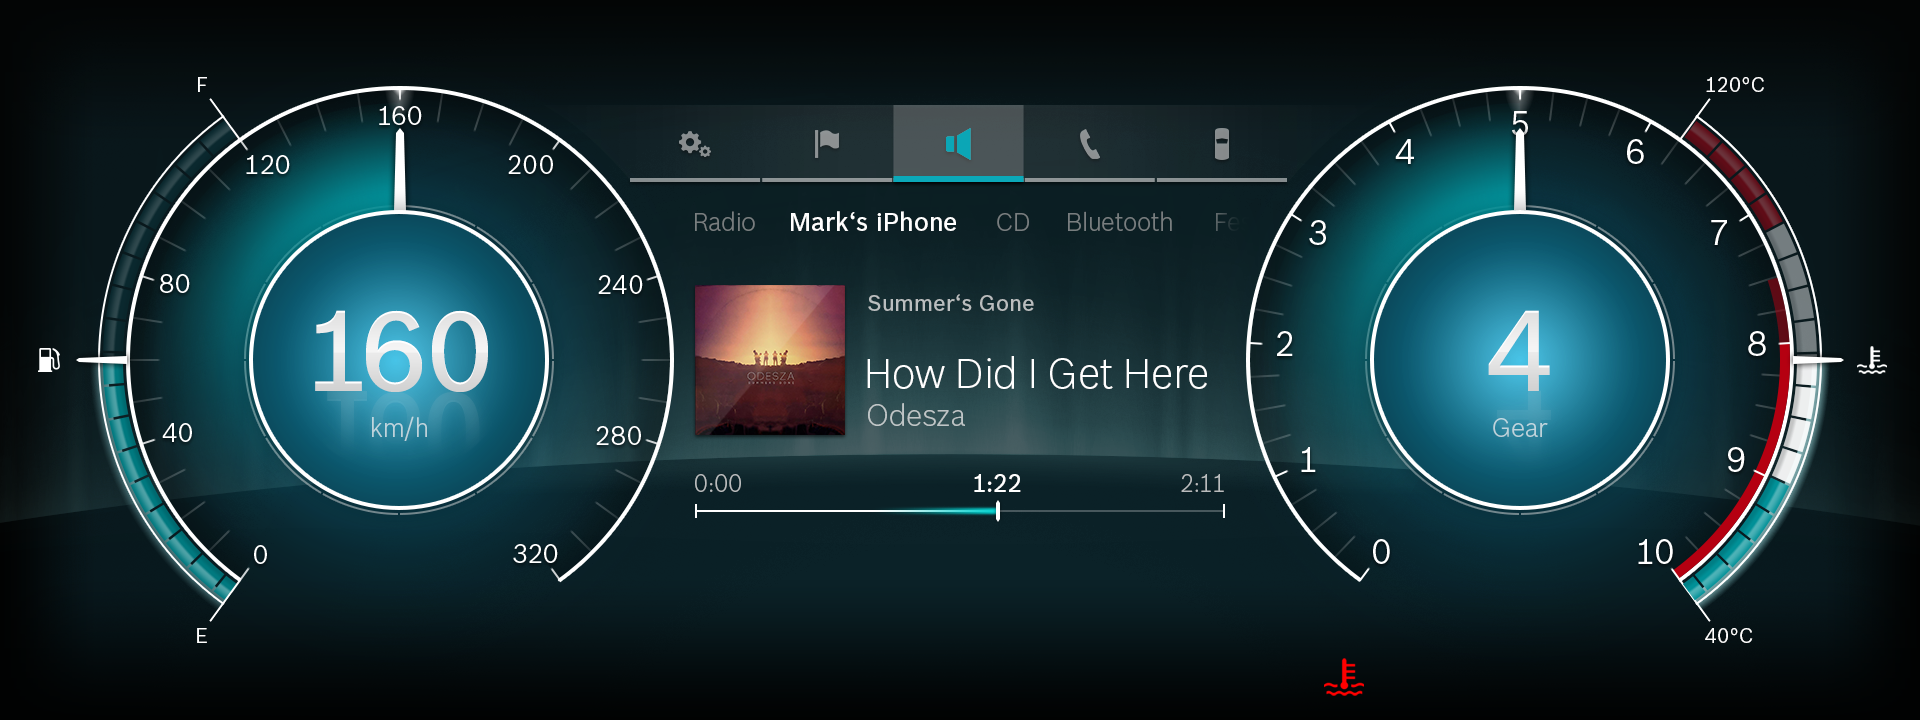
\includegraphics[width=\textwidth]{img/1_einleitung/beispielHMI}
	\caption[Beispielhaftes Instrument Cluster]{Beispielhaftes Instrument Cluster \cite{bosch}}
	\label{fig:hmi}
\end{figure}

% Erklärung zum Bild
Als Beispiel dient Abbildung \ref{fig:hmi}, dort ist eine Standardszene eines Kombiinstruments dargestellt. Links ist der Tachometer zu sehen. Die Geschwindigkeit wird einmal analog als Zeigerinstrument nachgebildet und einmal digital angezeigt. Links daneben befindet sich die Tankanzeige. Die rechte Seite zeigt die aktuelle Drehzahl und den aktuellen Gang an. Rechts daneben wird die Kühlwassertemperatur angezeigt. Die Mitte wird ausgefüllt von Multimedia-Funktionen wie Musik, Telefon und Navigation.\\

% Thema weiter erklären ->Entwicklung HMI Konzept
In der vorliegenden Arbeit, wird zunächst ein Architektur-Konzept entwickelt. Die Entwicklung dieses Konzepts umfasst die Recherche des aktuellen Stands sowie die Erstellung eines neuen Software-Architektur-Konzepts. Im Fokus stehen hierbei zum einen ein geringer Entwicklungs- und Kostenaufwand und zum anderen ein möglichst hohes Maß an Flexibilität. Der Entwicklungsaufwand, sowie die -kosten können durch standardisierte Software verringert werden. Diese Art der Software muss gleichzeitig einen großen Kreis an Kunden ansprechen um profitabel zu sein. Im Gegensatz dazu steht die individuelle Softwarelösung. Diese Art der Software erhöht Aufwand und Kosten. Deshalb gilt es ein Konzept zu finden das beide Ansätze optimal vereint.\\

%Architektur entwickeln
Eine Architektur zu entwickeln, ist ein umfangreicher Prozess. Damit dieser Prozess gelingt, müssen einige Dinge beachtet werden. So existieren zum Beispiel eine Reihe von ISO Normen die sich mit der Bewertung der Qualität von Software auseinandersetzen. Zudem gibt es verschiedene Designmöglichkeiten die sich gegenseitig ausschließen.\\

% Umsetzung des Konzepts
Für die Umsetzung des Konzepts gilt es als erstes eine grobe Architektur festzulegen. Danach muss die Entwicklungsumgebung ausgewählt werden. Die Software soll in jedem Fall wiederverwendbar sein, daher soll die Software möglichst aus Entwurfsmustern bestehen. Entwurfsmuster helfen, Software in einzelne wiederkehrende Muster aufzuteilen.\\

Die Auswahl an Entwicklungsumgebungen ist groß, daher muss hier eine Auswahl getroffen werden. Anschließend werden die Entwicklungsumgebungen getestet und müssen bewertet werden. Zur Wahl stehen hier CGI Studio, Storyboard und Qt. CGI Studio ist das aktuelle Entwicklungstool bei der Bosch Engineering GmbH. Hier soll eine mögliche Alternative gefunden werden, da zum einen die Einarbeitungszeit sehr hoch ist und zum anderen sind einige Funktionen sehr fehleranfällig. Sobald das Konzept fertig und die Entwicklungsumgebung gefunden ist, soll eine Prototypen-Software entwickelt werden. Damit soll gezeigt werden wie das Konzept umgesetzt werden kann.\\

%Ziele definieren
Das Ziel der Arbeit besteht zum einen aus der Erarbeitung einer Software-Architektur. Die Architektur soll den Entwicklungsaufwand für zukünftige Projekte zu reduzieren. Zum anderen muss ein dafür passendes Framework gefunden werden, mit dem die Architektur umgesetzt werden kann.\\

